\headline{{\textbf{\Large\sffamily Potting Shed Gossip:}}\\
          {\textbf{\large\sffamily Who's Ready for the New Talent Challenge?}}}
\label{2025-11-gossip}
\noindent
Last year, \textit{David Fishwick} and \textit{Mark Pittman} stepped boldly into the spotlight at the FoBBS New Talent Competition, and what a journey it was.
Their stories of grit, focus, and that wonderful mix of nerves and excitement still echo at our club meetings. 
They trained for months, packed their own tools and wire, and faced the ultimate test: transforming an unfamiliar tree under pressure while the judge circled like a hawk. 
As Mark said afterward, \textit{``When the judge hesitates, you know the work is good.''} 
They did Twickenham proud, and their experience proved that this competition truly is about learning, stretching your skills, and seeing what you're capable of.

Now it's \textit{\textbf{your}} turn.

The New Talent Competition (NTC) runs every year, and the British heat for 2026 will take place at \textbf{Bonsai Fest on 22 March in Newark}. 
The winner goes on to represent the UK at the European final, held in \textbf{Banská Bystrica, Slovakia, on 11 April 2026}, around 100 miles north of Budapest. 
Not only do you get to compete on the European stage, but your \textbf{flight and accommodation are covered}. 
Imagine that: your bonsai journey taking you all the way to central Europe!

The competition stays true to its roots: no professionals, no past winners — just raw, emerging talent. 
FoBBS provides the tree, you bring the skill and the courage. 
For those who felt inspired watching David and Mark step up last year, this is your chance to follow in their footsteps.

If you think you might want to give it a go, the entry form and full details are available at \url{fobbsbonsai.co.uk/newtalent.html}, and forms need to be returned to FoBBS by \textbf{30 January 2026}.

Interested? Curious? A tiny bit terrified but tempted anyway? Perfect. That's exactly how all great journeys start.

\textbf{Please speak to Chris Durne or Nick Lloyd at the next club meet-up}: they'll help gather names, guide you through the form, and make sure you're referred properly. 
Let's see if Twickenham can send another rising star (or two!) onto the national stage this year.
% 
Who's up for the challenge?

\begin{window}[2,l,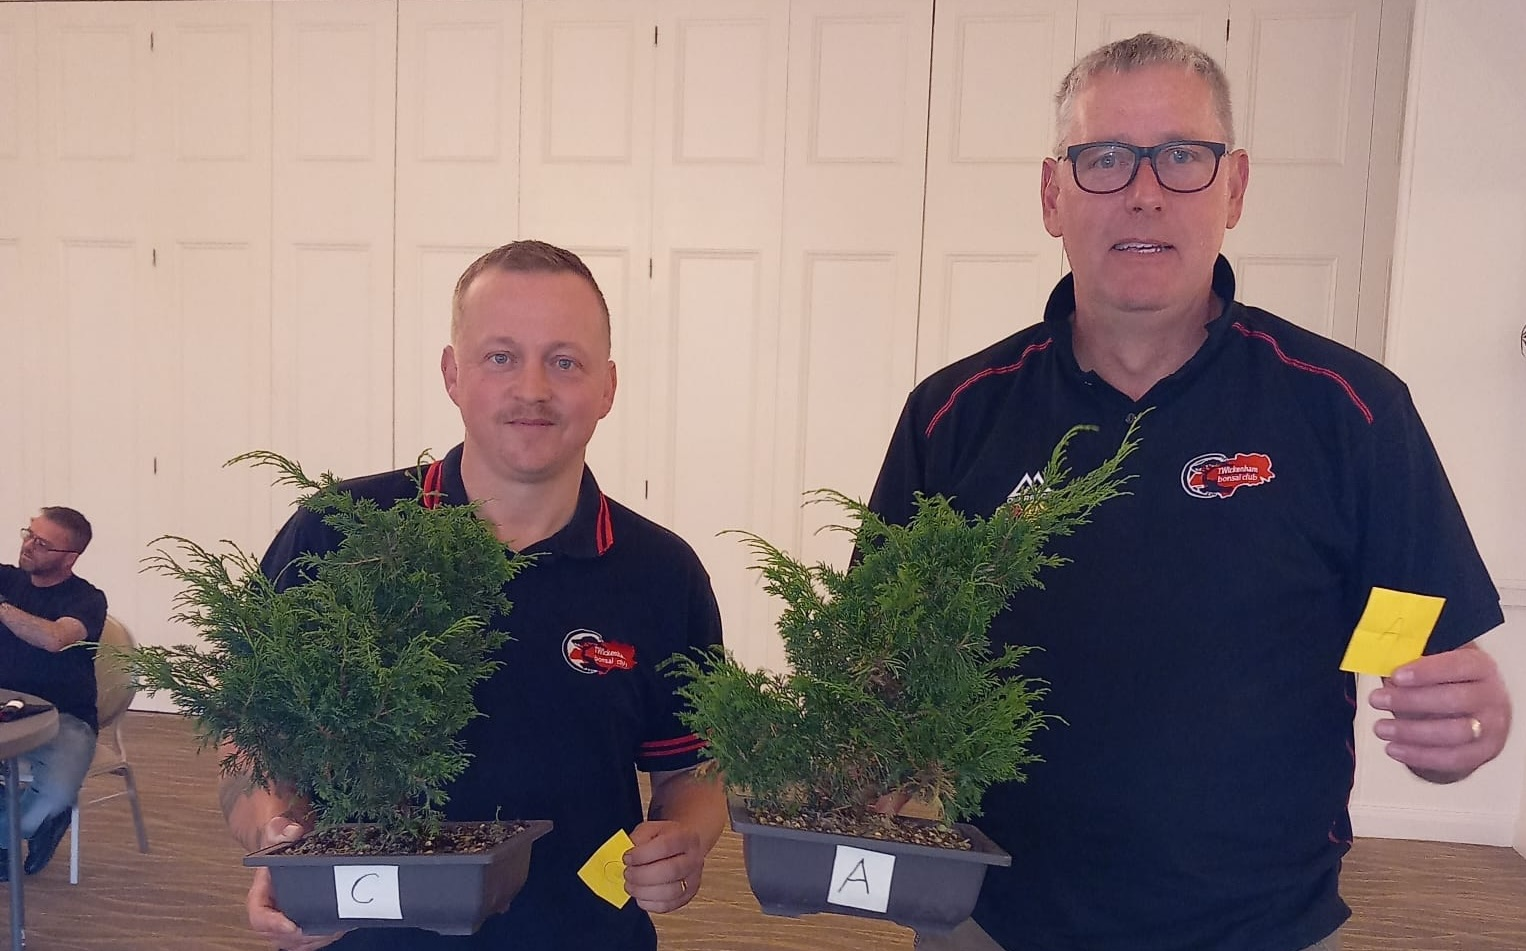
\includegraphics[width=1.0\columnwidth]{2025_11/res/gossip_ntc.jpg},\centerline{\emph{David and Mark at NTC 2025.}}]
\end{window}

\closearticle
\columnbreak